\documentclass[a4paper, 15pt]{article}
\usepackage[left=0.85in, right=0.85in, top=0.5in, bottom=0.95in]{geometry}
\usepackage[T1]{fontenc}
\usepackage[utf8]{inputenc}
\usepackage[italian]{babel}
\usepackage[none]{hyphenat} % no sillabazione 
\usepackage{multicol} %testo su più colonne
\usepackage{enumerate}
\usepackage{mdwlist} %suspend enumerate \suspend{} \resume{}
\usepackage{lipsum} %testo random per verifica \lipsum
\usepackage{graphicx, nicefrac}
\usepackage{wrapfig2}
\usepackage{amsmath}
\usepackage{mathtools}
\usepackage{amssymb}
\usepackage{amsthm} %teoremi e dimostrazioni e definizioni
\usepackage{gensymb} %simboli come ° = \degree  etc etc
\usepackage{cancel} %permette di fare semplificazioni utilizzando il comando \cancel{expression}
\usepackage{subcaption}
\usepackage{hyperref}
\hypersetup{
	colorlinks=true,
	linkcolor=blue,    
	urlcolor=blue,
	%pdfpagemode=FullScreen, %il pdf generato non si avvia a schermo intero
}
\urlstyle{same}
\usepackage{changepage}
\usepackage{lastpage, epstopdf}
\usepackage{fancyhdr}
\usepackage{tcolorbox}
%\usepackage{background} %non utilizza lo sfondo con "draft"
\usepackage{color} % testo colorato \textcolor{'ColorCode'}{'testo'}
\usepackage{setspace} % in questo modo posso settare lo spoazio dell'indice \begin{spacing}{0.95}
	\usepackage{changepage}
	\usepackage{lastpage, epstopdf}
	\usepackage{fancyhdr}
	\usepackage{tcolorbox}
	%\usepackage{background}
	
	%========SIUNIX========%
	\usepackage{siunitx}
	\DeclareSIUnit{\rpm}{rpm}
	
	%========TIKZ========%
	\usepackage{tikz} %disegni e mappe
	\usetikzlibrary{patterns}
	\usepackage{pgfplots}
	\pgfplotsset{compat=1.15}
	\usepackage{mathrsfs}
	\usetikzlibrary{arrows,decorations.markings}
	
	%========TEOREMI========%
	\newtheorem*{thm}{Teorema}
	\newtheorem*{en}{Enunciato}
	\newtheorem*{deff}{Definizione}
	\newtheorem*{cor}{Corollario}
	
	
	
	%========OPERATORI========%	
	\DeclareMathOperator{\rk}{rk}	
	\DeclareMathOperator{\im}{Im}
	\DeclareMathOperator{\ev}{ev}
	
	
	%=======HEADER & FOOTER=======%
	\def\lesson{Lezione N.25}
	
	
	\pagestyle{fancy}
	\fancyhf{}
	\renewcommand{\headrulewidth}{0pt}
	\renewcommand{\footrulewidth}{1.4pt}
	\lfoot{A.M. $\diamond$ \the\year}
	\cfoot{\thepage}
	\rfoot{\lesson}
	
	%=======BODY=======%
	\raggedbottom
	\setlength{\parindent}{0pt}
	\title{Parte 17: Ruote cilindriche}
	\date{}
	
	\begin{document}
		
		\maketitle
		\setcounterpageref{secnumdepth}{0}	
		\tableofcontents 
		\newpage
		
		\section{Limiti di ingranamento}		
		\begin{adjustwidth}{2in}{} 
		Il dimensionamento geometrico prima di tutto deve essere funzionale, cioè deve garantire il corretto funzionamento dell'ingranaggio, affinché questo avvenga è perciò necessario evitare condizioni di contatto reciproco fra i denti fuori dalle condizioni standard di profili coniugati.
		
		Si ipotizzi allora una dentatura ad evolvente, la condizione affinché si abbia una profilo efficace al contatto esclusivamente ad evolvente è la presenza di una circonferenza fondamentale (o di base), interna alla circonferenza di piede: solo in questo modo si avrà che tutto il profilo utile segue il profilo ad evolvente. 
		\begin{figure}[H]
			\centering
			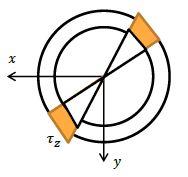
\includegraphics[width=0.5\linewidth]{immagini/screenshot001}
			\label{fig:screenshot001}
		\end{figure}
		Esiste una relazione che permetta di affermare con sicurezza che la circonferenza fondamentale sia al disotto di quella di piede?
		
		A partire dal proporzionamento unificato, quindi da un dente con un addendum pari al modulo ed un dedendum pari a ${5\over4}$ del modulo,  affinché il profilo del dente sia tutto all'esterno della circonferenza fondamentale si dovrà imporre che la differenza tra raggio di primitiva e raggio di fondamentale sia maggiore o uguale a ${5\over4}$ del modulo. 
		\[u = 1.25m = {5\over4}m\]
		Tale relazione, ricordando che dedendum è la distanza radiale tra la circonferenza fondamentale e quella di piede, si può scrivere come 
		\[{5\over4}m\leq R - \rho = R(1-\cos\theta)\]
		Dal fatto che $\rho=R\cos\theta$ con $\theta$ angolo di pressione. \newline 
		
		Poiché il numero di denti è in relazione al modulo e al raggio secondo 
		\[m = \dfrac{2R}{z}\] 
		Allora il numero di denti $z$ minimo affinché la circonferenza fondamentale sia al di sotto della circonferenza di piede è
		\[z\geq \dfrac{\nicefrac{5}{2}}{1-\cos\theta}\]
\newpage		
		L'obiettivo prefissato è quello di dimensionare un ingranaggio che sia funzionale e che cioè massimizzi il più possibile il fattore di ricoprimento, questo significa garantire due condizioni:
		\begin{enumerate}
			\item In ogni istante un fattore di ricoprimento maggiore di 1
			\item L'assenza di condizioni critiche di interferenza
		\end{enumerate} 
		Al tempo stesso però la buona pratica ingegneristica suggerisce in più di individuare soluzioni compatte e di dimensioni contenute per ridurre ingombri, masse e aumentare le prestazioni massime, allora talvolta sarà necessario porsi al di sotto di questo numero di denti.
		
		Questo perché in un dimensionamento proporzionale un numero di denti che cresce equivale a dimensioni che crescono: fissato un modulo, se cresce il numero di denti aumenta giocoforza il diametro della ruota. \newline 
		
		Poiché il valore del modulo è dettato da considerazioni di resistenza, diminuire le dimensioni significa porsi al disotto di questo limite, il che si può fare tenendo bene a mente le conseguenze:
		\begin{enumerate}
			\item La fondamentale cadrà al di sopra del piede
			\begin{enumerate}
				\item Il segmento dei contatti diminuirà
				\item Possibilità di un fattore di ricoprimento $<1$
			\end{enumerate}
			\item Per evitare il contatto coniugato testa/piede diviene necessaria opportuna fresatura
		\end{enumerate}		
		A volte la decisione di prolungare il profilo del dente oltre la circonferenza di base potrebbe essere strategico, si può infatti decidere di lavorare con tratti rettilinei, come in figura il tratto $BB'$
		\begin{figure}[H]
			\centering
			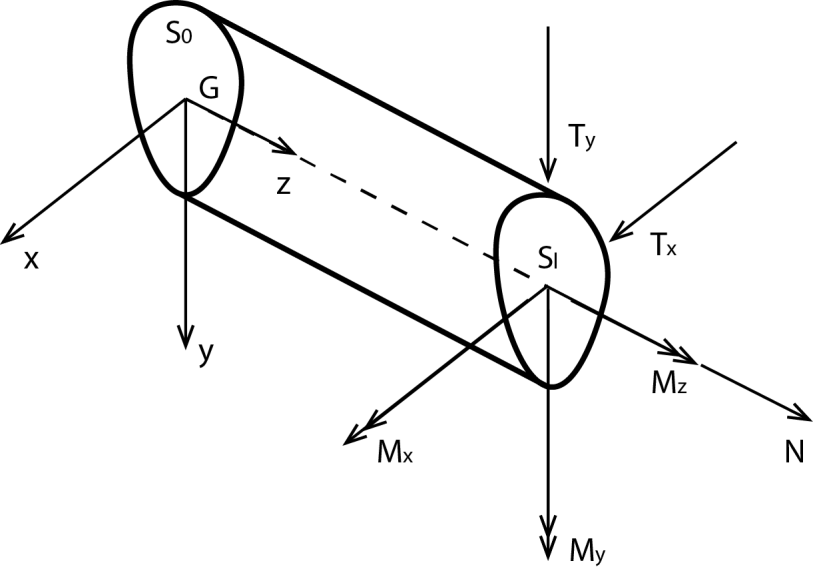
\includegraphics[width=0.5\linewidth]{immagini/screenshot002}
			\label{fig:screenshot002}
		\end{figure}
		Si può o sfruttare una parte del profilo del dente oltre l'evolvente, oppure prevedere di tagliare il profilo, scavandolo al di sopra della circonferenza di base in modo da evitare il contatto della dentatura nella zona prossima alla circonferenza fondamentale: lì infatti il profilo arriva con una pendenza che ha una tangente in B perfettamente radiale: dalla distribuzione delle velocità è noto che esistano ha una velocità normale al profilo ed una velocità tangenziale ad esso; la componente normale è quella con cui si muove il punto di contatto lungo il segmento dei contatti, mentre quella tangenziale è invece quella che permette lo scorrimento dei profili, quella che porta usura e grippaggio. 
		
		Per cui se il contatto avviene in prossimità del punto B la velocità è quasi esclusivamente tangenziale: lì è dove si massimizza l'effetto di usura e strisciamento, per cui se ci si può permettere di perdere un po' di segmento dei contatti (= ho un fattore di ricoprimento molto superiore ad 1 e quindi lo posso sacrificare), allora si preferisce perdere quella porzione che porterebbe solo problemi dal punto di vista resistenziale, e scavarlo così da evitare il contatto. 
		
		Infatti lì il contatto si avrebbe per puro cinematismo, per cui se si asporta il materiale il dente coniugato non troverà parte del profilo e il contatto ripartirà esattamente dove ricomincerà il profilo ad evolvente. 
\end{adjustwidth}
\newpage
\section{Interferenza}		
\begin{adjustwidth}{2in}{} 		
		L'interferenza è l'atto e l'effetto dell'incontro tra profili in un punto del meccanismo in cui tali profili hanno normali non comuni, cioè hanno atti di movimento aventi ciascuno la direzione propria.
		\begin{figure}[H]
			\centering
			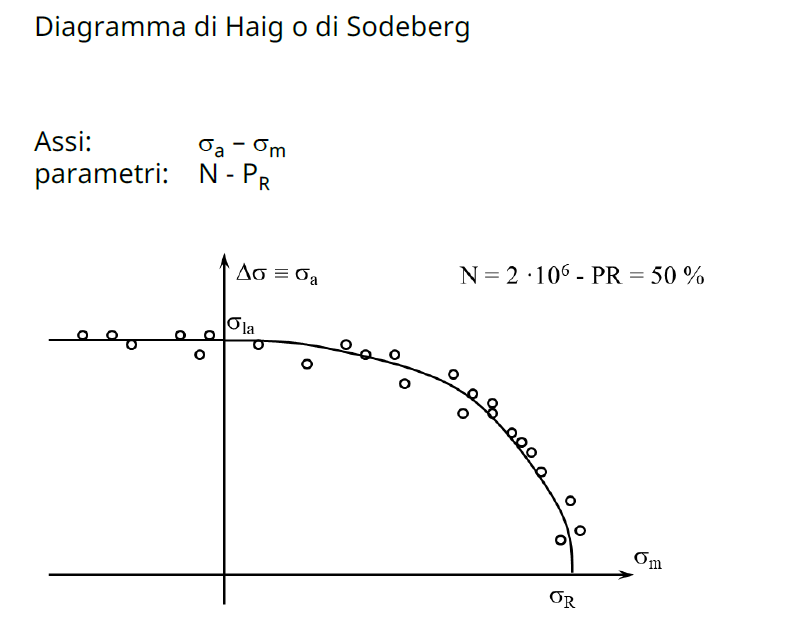
\includegraphics[width=0.5\linewidth]{immagini/screenshot003}
			\label{fig:screenshot003}
		\end{figure}		
		Se il contatto avviene sui punti del segmento dei contatti compresi fra $T_1$ e $T_2$, segmento teorico del contatti tra i punti di tangenza della retta d'azione con le fondamentali, sarà un contatto certificato tra profili coniugati con la sicurezza che non avvenga interferenza.
		
		Questa infatti è una condizione che durante l'ingranamento è non si deve mai verificare, qualunque sia la sua tipologia o entità. \newline
		
		L'avvento dell'interferenza tra profili durante il funzionamento di un ingranaggio porta al bloccaggio istantaneo dello stesso, con conseguente danneggiamento di tutti gli organi collegati.
		
		Questo impuntamento è dovuto al fatto che nel punto di contatto le due ruote hanno velocità incompatibili e l'atto di moto sviluppa la tendenza alla compenetrazione. 
		
		In fase di realizzazione, al contrario, è possibile ammettere un particolare tipo di interferenza al fine di scavare il profilo del dente. \newline
			
		Qualunque tipo di interferenza è in condizioni teoriche del tutto prevedibile per via geometrica. 
		
		Le due tipologie principali di interferenza che si hanno nello studio delle ruote dentate cilindriche esterne sono
		\begin{enumerate}
			\item L'interferenza teorica, primaria, d'evolvente
			\item L'interferenza di raccordo
		\end{enumerate}
		Sono tipologie di interferenza perfettamente ricostruibili geometricamente, sono dettate dal cinematismo ideale del sistema e consistono sostanzialmente nel verificare che il contatto effettivo avvenga all'interno di un determinato segmento dei contatti, questo segmento dei contatti, a seconda che lo consideri individuato dalle troncature esterne o da quelle di testa o di piede definisce una  condizione piuttosto che l'altra. 
\end{adjustwidth}
\newpage
\subsection{Interferenza primaria o interferenza di evolvente}		
\begin{adjustwidth}{2in}{} 		
		Questa è causata dalla possibilità di avere un punto di contatto tra i profili esterni al segmento teorico del contatti. 
		\begin{figure}[H]
	\centering
	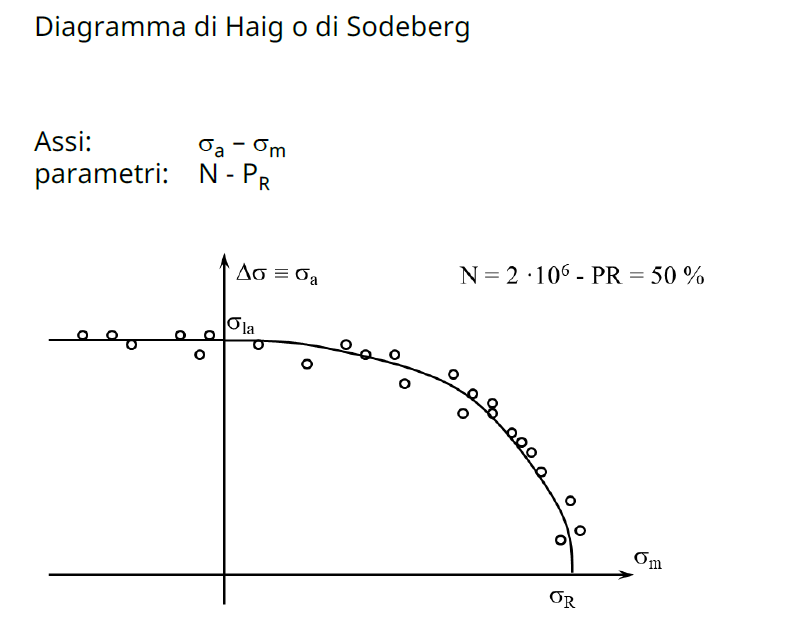
\includegraphics[width=0.5\linewidth]{immagini/screenshot003}
	\label{fig:screenshot003.bis}
		\end{figure}		
		Si ricordi a questo proposito come si era definito tale segmento teorico dei contatti, era $T_1T_2$ individuato dalle tangenze della retta d'azione con le circonferenze di base di ruota e pignone. 
		
		Se si avessero i punti di contatto al di fuori di quel segmento, vorrebbe dire che si verificherebbe un contatto fuori dal profilo ad evolvente: $T_1$ rappresenta infatti il punto minimo di evolvente del pignone e $T_2$ il minimo della ruota, ora se la circonferenza di testa della ruota toccasse il profilo ad evolvente del pignone al di fuori di $T_1$ cioè fosse più sporgente del raggio $O_2T_1$, allora si verificherà  interferenza di evolvente.\newline 
		
		Osservando ad esempio il punto $P$, questo appartiene al segmento dei contatti.
		
		Se la troncatura esterna del pignone è maggiore di $T_1T_2$ e arriva fino a P, significherebbe avere un raggio di testa del pignone $O_1P$ - per garantire il contatto in P - ben oltre il punto $T_2$, ben oltre il possibile contatto sul profilo ad evolvente.
		
		D'altronde per definizione di profili coniugati, nel punto di contatto si devono avere sempre due profili con la stessa tangente, con la stessa normale. 
		
		Si vede così che al profilo $p1$ del dente ad evolvente del pignone che toccherebbe in P il profilo coniugato non corrisponde alcun evolvente di ruota tangente, se non quel $p2'$, che però ha la stessa concavità di $p1$ e quindi la spinta sul dente non avverrebbe correttamente: quello non è un profilo utile di contatto, può essere al massimo un profilo ozioso, il profilo utile sarebbe il simmetrico di quel ramo di evolvente, cioè $p2$.
		\begin{figure}[H]
	\centering
	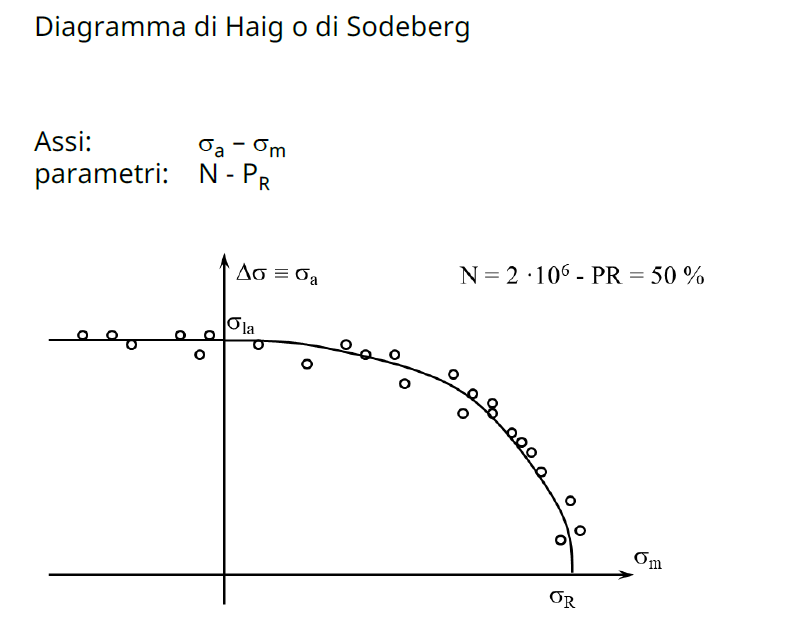
\includegraphics[width=0.3\linewidth]{immagini/screenshot003.2}
	\label{fig:screenshot003.2}
		\end{figure}				
		Zoomando di vede però che $p2$ è intersecante $p1$: il punto $R$ è più a sinistra del punto $Q$, i due rami di evolvente si intersecano, lì avviene interferenza.
\newpage				
		Verificare che non ci sia questo tipo di interferenza è banale: si deve verificare che i segmenti effettivi dei contatti in accesso e rispettivamente in recesso siano sempre inferiori al segmento teorico dei contatti, quindi se si individuano i punti $A$ ed $E$ come punti di intersezione delle troncature esterne di ruota e pignone col segmento \textit{teorico} dei contatti è più che noto che questi definiscano il segmento \underline{effettivo} dei contatti. 		
		\begin{figure}[H]
			\centering
			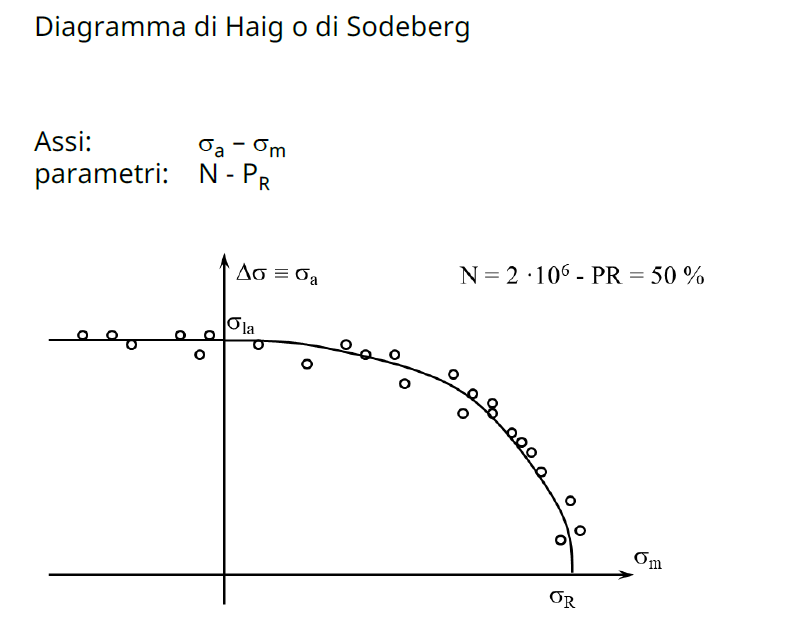
\includegraphics[width=0.5\linewidth]{immagini/screenshot003.3}
			\label{fig:screenshot003.3}
		\end{figure}
		Si dovrà verificare allora che il segmento $CE$ sia inferiore a $CT_2$, e che il segmento $CA$ sia inferiore a $CT_1$, e quindi che il punto di intersezione del segmento dei contatti con le troncature esterne ricada all'interno del segmento teorico massimo dei contatti $T_1T_2$. 
		\[CE<CT_2\qquad CA<CT_1\]		
		Questa verifica è molto più stringente al crescere del numero di denti della ruota e al ridursi di quelli del pignone: aumentando la differenza del numero di denti questa verifica diventa più critica. \newline
		
		In sostanza è l'addendum della ruota ad essere l'autore di interferenza sul dedendum del pignone, allora per evitare l'interferenza si può lavorare sul proporzionamento di ruota e pignone; l'ideale sarebbe aumentare l'addendum del pignone e ridurre l'addendum della ruota, seguendo questa linea di principio si otterrebbe, a parità di interasse  e numero di denti, un aumento del circa 30\%  del segmento dei contatti, il problema è che questo espediente con un proporzionamento unificato non si può applicare, semplicemente perché l'addendum è pari al modulo non si può fuggire da quella condizione, se non optare per ruote dentate \textbf{corrette}. 
		\begin{figure}[H]
			\centering
			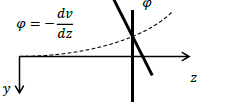
\includegraphics[width=0.3\linewidth]{immagini/screenshot004}
			\label{fig:screenshot004}
		\end{figure}		
		Simultaneamente si potrebbe lavorare sugli addendum di ruota e pignone, oppure sull'angolo di pressione; infatti riducendo l'angolo di pressione si riescono a spostare i punti di contatto in modo da avere una condizione più favorevole alla non interferenza: sostanzialmente si stanno spostando i punti $T_1T_2$; al tempo stesso però, riducendo l'angolo di pressione, si riduce anche il segmento dei contatti: è un gioco di proporzioni di ottimo che come progettista si dovranno andare a ricercare.
\end{adjustwidth}
\newpage
\subsection{Interferenza di raccordo}		
\begin{adjustwidth}{2in}{}
		L'altro tipo di interferenza e quella di raccordo. 
		
		Questa si verifica quando la circonferenza di base si trova al di sotto della troncatura interna o del piede. \newline
		
		L’interferenza di raccordo consiste nella condizione che la testa dei denti della ‘ruota’ vada a “mordere” il tratto
		rettilineo del fianco dei denti del pignone o quello di raccordo del dente con la superficie di radice. \newline
		
		In generale l'interferenza si verifica quando un punto del profilo non è ad evolvente ed è noto che alla base di ogni dente c'è sempre un raggio di raccordo non ad evolvente.
		
		La condizione per evitare quindi interferenza di raccordo prevede così che non ci sia contatto su quella parte di profilo, che per costruzione è superiore alla circonferenza di base.
		
		Si chiama \textbf{interferenza di raccordo positiva} quella in cui si ha un contatto sul raggio di raccordo; se invece si assiste ad un contatto nella zona rettilinea creata sul profilo mediante fresatura, allora quella è una \textbf{interferenza di raccordo negativa}. \newline 
		
		In pratica si può estendere la verifica precedentemente descritta per l'interferenza primaria andando a valutare le troncature esterne e interne anziché le circonferenze di piede e di testa. 
		
		In questo modo un ulteriore limitazione al segmento dei contatti teorico si ottiene andando ad introdurre le troncature esterne ed interne, ovvero le circonferenze che passano per il primo e l'ultimo punto del profilo ad evolvente del dente. \newline
		
		Talvolta però, tale interferenza di raccordo  - che deve essere sempre evitata in un funzionamento dell'ingranaggio - può essere ricercata durante il taglio stesso della ruota dentata. 
		
		Questo meccanismo infatti permette il contatto (e quindi l'eliminazione, viene scavata via) di quella porzione sulla quale si avrebbe avuto un profilo ad evolvente esteso fino alla circonferenza di base che avrebbe causato, proprio per interferenza di raccordo, pitting e usura.
		\begin{figure}[H]
			\centering
			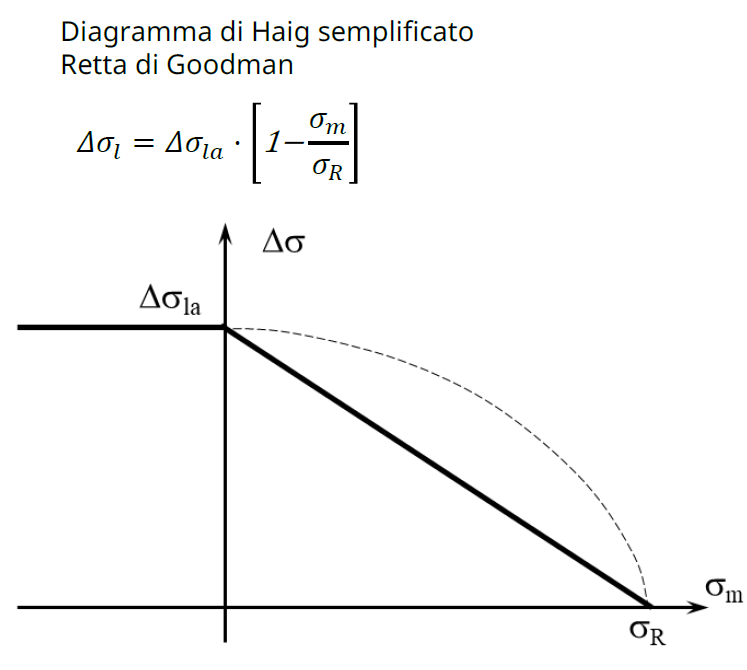
\includegraphics[width=0.5\linewidth]{immagini/screenshot005}
			\label{fig:screenshot005}
		\end{figure}				
		Tuttavia la conseguenza che si deve tenere in considerazione con lo scavo del dente è il fatto che questa nuova circonferenza, chiamata circonferenza di interferenza, cioè quella circonferenza che passa per l'ultimo punto utile dell'evolvente, diventa il nuovo limite del segmento dei contatti effettivo: sarà infatti l'ultimo possibile punto di contatto sul segmento dei contatti. 
		\begin{figure}[H]
			\centering
			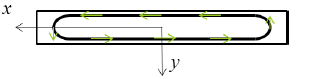
\includegraphics[width=0.5\linewidth]{immagini/screenshot006}
			\label{fig:screenshot006}
		\end{figure}		
		Anche in questo caso, per evitare l'interferenza di raccordo si agisce aumentando il più possibile la denatura del pignone o riducendo quella della ruota. 
		
		Anche se da una parte il taglio della base del dente migliora la resistenza ad usura, dall'altra riduce la radice del dente e quindi st sta riducendo la resistenza a flessione del dente: è un intervento che deve essere realizzato sempre \textit{cum grano salis}. 
\end{adjustwidth}
%\newpage
\section{Numero minimo di denti}		
\begin{adjustwidth}{2in}{} 
		Si può quantificare l'intervento appena proposto andando a ragionare il numero minimo i denti di funzionamento durante il cinematismo affinché sia scongiurato l'effetto dell'interferenza. \newline 
		
		Per evitare qualunque tipo di interferenza di raccordo che sia negativa o positiva, esiste una relazione geometrica che quantifica il numero minimo di denti di ruota e pignone affinché il cinematismo di funzionamento o quello di taglio, possa avvenire; ovvero un numero minimo di denti che garantisca un fattore di ricoprimento maggiore di 1 e una non interferenza. \newline 
		
		Se si applica al cinematismo ruota-pignone, questo si configura essere il numero minimo di denti dell'intero cinematismo.
		
		Siccome questa trattazione considera solo riduttori di velocità, si tratterà allora del numero minimo di denti che il pignone deve giustificare.
		
		Se invece lo si applica all'accoppiamento rocchetto-dentiera, è il numero minimo di denti della ruota che si sta realizzando.\newline 
		
		Allora, per coppie a dentatura esterna il numero minimo di denti in un accoppiamento ruota pignone è
		\[z_{min} \geq \dfrac{2k'\tau}{\sqrt{1+\tau(2+\tau)\sin^2\theta}-1} =2k' \dfrac{1+\sqrt{1+\tau(1+\tau)\sin^2\theta}}{(2+\tau)\sin^2\theta}\]
		Ed il fattore di ricoprimento diviene 
		\[\varepsilon = \dfrac{1}{2\pi}\left[\sqrt{\left(\dfrac{z'+ 2k'}{\cos\theta}\right)^2-z'^2} + \sqrt{\left(\dfrac{z+ 2k}{\cos\theta}\right)^2-z^2} -(z+z')\tan\theta \right]\]
		Per una coppia rocchetto-dentiera si realizza un numero minimo di denti pari a
		\[z_{min} \geq \dfrac{2k'}{\sin^2\theta}\]
\newpage		
		Le relazioni che si leggono derivano da tutte le considerazioni geometriche descritte finora. \newline 
		
		$z$ è il numero minimo di denti tra pignone e ruota, $k'$ è il coefficiente numerico da assegnare all'addendum della specifica ruota.
		
		Quindi se si sta parlando del pignone, $k'$ è l'addendum della ruota, che in un proporzionamento unificato vale 1. 
		
		$\tau$ è il rapporto di trasmissione, $\theta$ è l'angolo di pressione. \newline
		
		Se nella relazione del numero minimo di denti si usa un \textbf{rapporto di trasmissione nullo}, ovvero quello che si ha tra rocchetto e dentiera, si ottiene il numero minimo di denti realizzabile dall'accoppiamento cinematico di realizzazione.
		
		Perché $\tau=0$ nella realizzazione? La polare di una dentiera è una retta che rotola su una circonferenza, ma una retta ha raggio di curvatura infinito e quindi il rapporto tra i raggi che effettivamente fornisce il rapporto di trasmissione è nullo.
		
		Il numero minimo di denti intagliabile dipende così dall'anglo di pressione e dalla sporgenza della ruota coniugata, ovvero dalla dentiera: quanto sporge dalla primitiva il dente della dentiera in addendum, tanto scaverà in dedendum. \newline
		
		La relazione che fornisce il \textbf{fattore di ricoprimento} si poteva tranquillamente calcolare come il rapporto tra il segmento effettivo dei contatti ed il prodotto tra il coseno di $\theta$ ed il passo. \newline 
		
		Le due prime relazioni sul numero di denti si possono riportare in un diagramma dove si può valutare il $k'$ dell'utensile unitario. 
		
		A questo proposito viene riportato il valore del minimo numero di denti intagliabile in funzione dell'angolo di pressione.
		\begin{figure}[H]
			\centering
			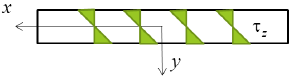
\includegraphics[width=0.4\linewidth]{immagini/screenshot007}
			\label{fig:screenshot007}
		\end{figure}		
		Come è possibile notare, il numero minimo di denti intagliabile nella fase di inviluppo, ovvero quella caratterizzata da un rapporto di trasmissione nullo, è un numero che dipende, una volta fissato $k'$, esclusivamente dall'angolo di pressione; il tipico angolo di pressione in un proporzionamento normale è \SI{20}{\degree}, quindi per rapporto di trasmissione nullo si avranno all'incirca 17 $\div$ 18 denti, ovvero il numero minimo di denti intagliabile senza interferenza di raccordo. 

		Per le ruote esterne ($\tau>0$) il numero minimo di denti intagliabili - per 20 gradi - è minore: si possono avere dei pignoni da 12 $\div$ 14 denti e dal punto di vista del cinematismo di funzionamento si avrebbero meno denti di quelli ottenuti per inviluppo, il problema è che per ottenerli si dovrà utilizzare una tecnologia diversa da quella dell'inviluppo con dentiera, come ad esempio la fresatura, con tutti i possibili svantaggi che ne derivano dal punto di vista dei costi e della produzione in serie.
		\newpage 
		Si nota poi che aumentando l'angolo di pressione si ottiene che il numero di denti minimo realizzabile decresce molto: se si vuole un ingranaggio più compatto sarebbe auspicabile lavorare con un angolo di pressione maggiore dei \SI{20}{\degree} canonici.
		
		Perché non si superano i \SI{30}{\degree}? Perché significherebbe avere ho lo stesso carico radiale di quello utile: si stanno scaricando sull'albero delle forze enormi, ad ingranaggi di piccole dimensioni corrispondono sempre alberi di grosso taglio per resistere ai forti carichi. 
		
		Al tempo stesso, avere un pignone con pochissimi denti induce problemi per quanto riguarda il fattore di ricoprimento, ridurre il numero di denti comporta una pericolosa riduzione all'unità del fattore di ricoprimento.
\end{adjustwidth}
%\newpage
\subsection{Taglio del dente}		
\begin{adjustwidth}{2in}{} 
		La tecnologia storica è quella per asportazione di materiale mediante fresa, con utensili a bottone (2) o a disco (1).
		\begin{figure}[H]
			\centering
			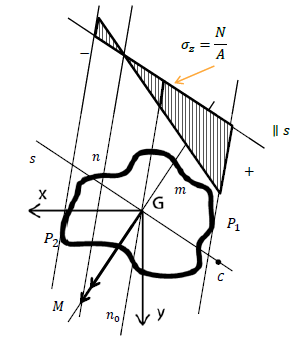
\includegraphics[width=0.3\linewidth]{immagini/screenshot008}
			\label{fig:screenshot008}
		\end{figure}		
		 I principali svantaggi sono 
		 \begin{itemize}
		 	\item Si scava un dente per volta
		 	\item L'utensile deve avere l'\underline{esatta} forma del vano
		 \end{itemize}
		Con una maggiore flessibilità ma con una minore precisione, si faceva uso del taglio per fresatura mediante sagoma, si utilizzava cioè una proporzione con un prototipo di grandi dimensioni e sfruttando l'effetto scala di una leva si faceva scorrere l'utensile sulla sagoma ed un utensile al raggio minore scavava il profilo del dente.
		\begin{figure}[H]
			\centering
			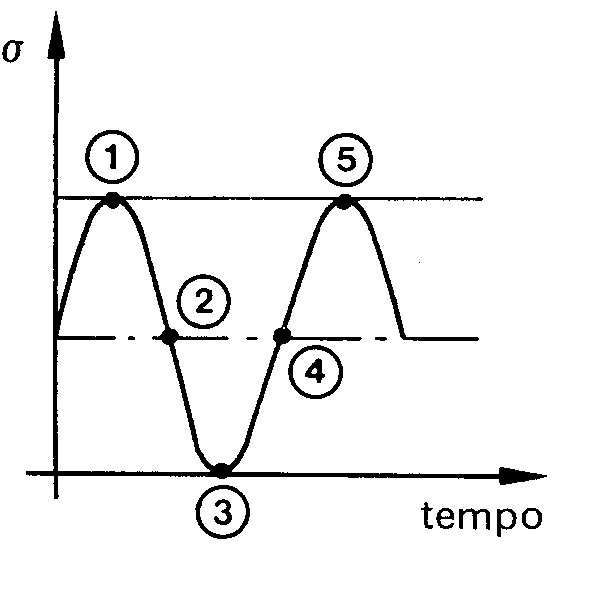
\includegraphics[width=0.5\linewidth]{immagini/screenshot009}
			\label{fig:screenshot009}
		\end{figure}		
		Tutti questi profili di \textbf{taglio diretto} della dentata sono tecnologie che non vanno d'accordo con la produzione in serie: è un processo lento, dente per dente e poco esatto. L'accoppiamento cinematico è di un utensile che si muove su di una ruota ferma. \newpage
		Tecnologia decisamente più favorevole alla produzione in serie è quella del \textbf{taglio indiretto} o taglio per inviluppo, in cui il taglio della ruota avviene mediante un azione simultanea  di rotazione e di moto del tagliante e del tagliato, dell'utensile e del rocchetto. L'utensile ora ha una forma differente da quella del vano scavato perché scava in funzione della posizione reciproca che durante l'ingranamento questo assume. \newline 
		
		l'utensile per inviluppo può essere di vario tipo, come una \textbf{generatrice (o stozzatrice) Fellows}, questa altri non è che una ruota dentata con degli utensili taglienti sugli estremi del profilo, nel moto relativo scava il profilo del dente asportando il materiale e creando il vano. 
		
		Il proporzionamento di addendum e dedendum è naturalmente invertito rispetto all'oggetto che si vuole realizzare, e quindi la sporgenza, l'addendum della generatrice, è pari al dedendum della generata e viceversa.
		\begin{figure}[H]
			\centering
			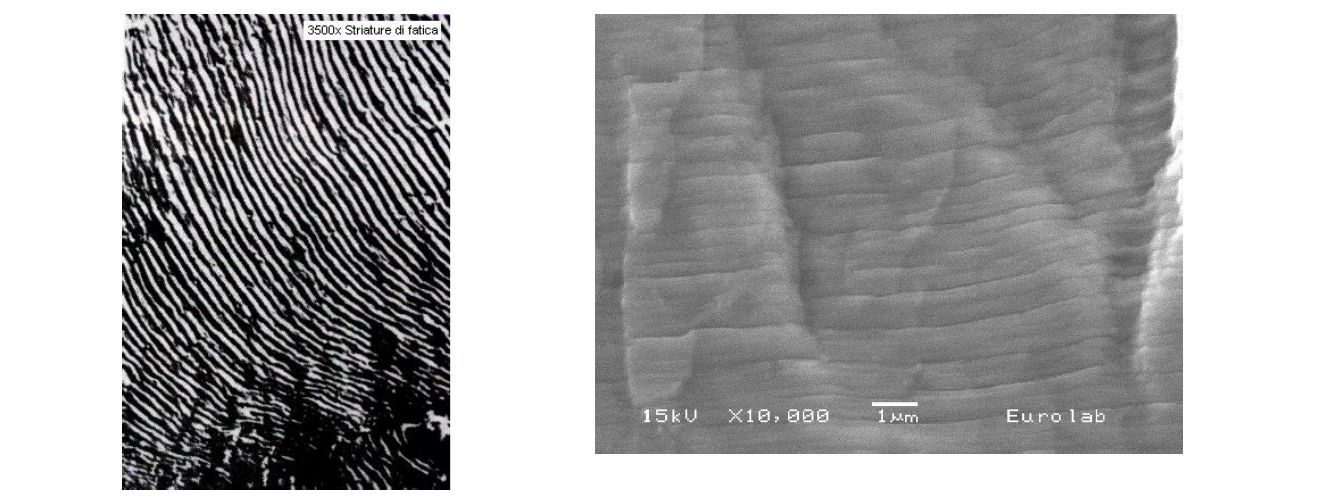
\includegraphics[width=0.5\linewidth]{immagini/screenshot010}
			\label{fig:screenshot010}
		\end{figure}
		Lo stesso concetto diviene applicabile con più elasticità nel caso in cui si immagina, anziché un rotolamento relativo di due circonferenze primitive, un moto relativo di una circonferenza primitiva con una retta primitiva (circonferenza dal raggio infinito), ovvero accoppiando un moto di traslazione con un moto di rotazione. 
		\begin{figure}[H]
			\centering
			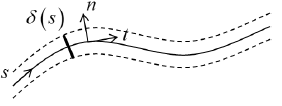
\includegraphics[width=0.5\linewidth]{immagini/screenshot012}
			\label{fig:screenshot012}
		\end{figure}
		Ogni punto del profilo dell'utensile genera dei rami di evolvente, l'utilizzo di una \textbf{dentiera utensile MAAG} permette di scavare il profilo ad evolvente accoppiando un cinematismo di traslazione e rotazione della ruota da tagliare.
		\begin{figure}[H]
			\centering
			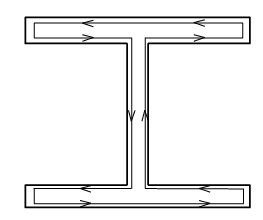
\includegraphics[width=0.5\linewidth]{immagini/screenshot011}
			\label{fig:screenshot011}
		\end{figure}		
		Poi attraverso l'opportuna sagoma della testa della dentiera si possono realizzare il raggio di raccordo alla base, le spoglie di testa e di piede, \dots \newline
		
		La dentiera, durante l'ingranamento, per poter scavare tutta la larghezza di fascia, cioè la profondità assiale della ruota dentata, lavora asportando il materiale anche in direzione assiale. 
		
		Se si immagina allora di accoppiare questo moto traslatorio ad uno rotatorio, e quindi si immagina che la dentiera anziché muoversi assialmente ruota intorno ad un asse di rotazione ortogonale all'asse della ruota da realizzare, si genera l'utensile \textbf{creatore}.  
		\begin{figure}[H]
			\centering
			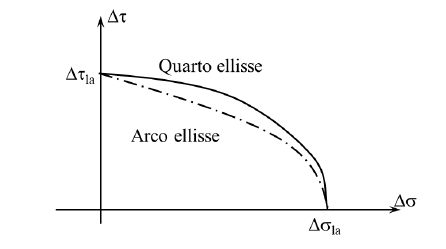
\includegraphics[width=0.5\linewidth]{immagini/screenshot013}
			\label{fig:screenshot013}
		\end{figure}
		Questo utensile non è altro che una rivoluzione della dentiera in cui si permette l'asportazione di truciolo accoppiando questa rivoluzione con un moto che si svolge lungo un'elica, interrompendo circonferenzialmente l'utensile da dei taglianti, in modo da smaltire truciolo. \newline
		
		Ecco come si delinea la proporzione tra dentiera e profilo scavato: ho bisogno di un dedendum della ruota scavata pari a 1.25 volte il modulo, allora l'addendum della dentiera deve essere pari ad 1.25 volte il modulo.
		\begin{figure}[H]
			\centering
			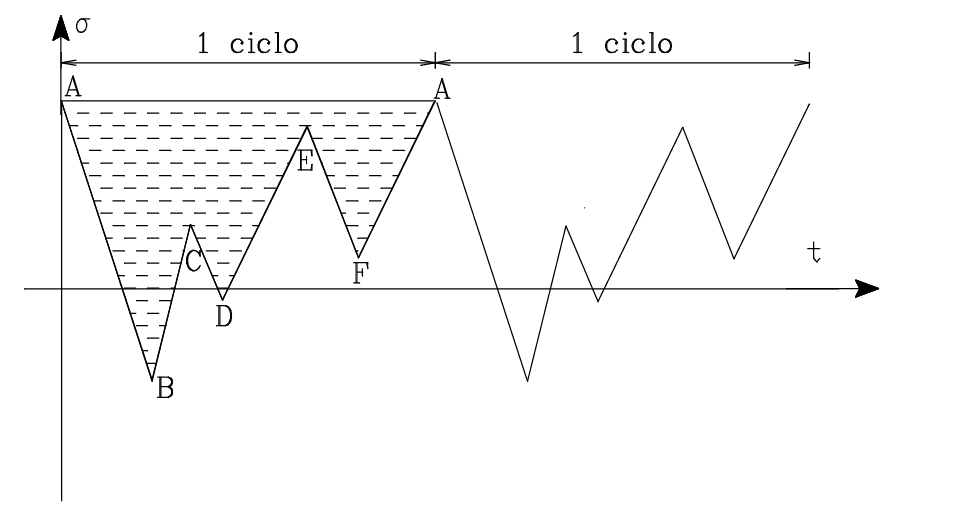
\includegraphics[width=0.5\linewidth]{immagini/screenshot014}
			\label{fig:screenshot014}
		\end{figure}		
		La dentiera scava con la sua testa anche il raggio di raccordo, per evitare problemi di contatto tra il piede della dentiera e la testa del rocchetto anche il dedendum è pari a 1.25 volte il modulo anche se il profilo effettivo da scavare è 1 volta il modulo, si garantisce sempre un certo gioco in testa scegliendo opportunamente il rocchetto di partenza: non si va a scavare la testa del rocchetto, dovrei avere il tagliente anche sul piede della dentiera.
		\begin{figure}[H]
			\centering
			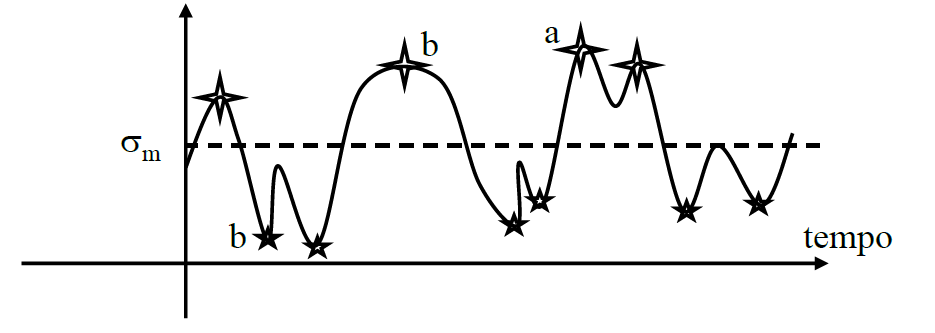
\includegraphics[width=0.5\linewidth]{immagini/screenshot015}
			\caption{Alcune realizzazioni mediante dentiera}
			\label{fig:screenshot015}
		\end{figure}
		Nel caso in cui i denti della dentiera siano inclinati si ottiene una dentatura elicoidale, altrimenti si ottiene una ruota dentata a denti dritti, l'utensile scava lungo la lunghezza d'asse. \newline 
		
		Per evitare il moto d'accostamento si utilizza il creatore.
		\begin{figure}[H]
			\centering
			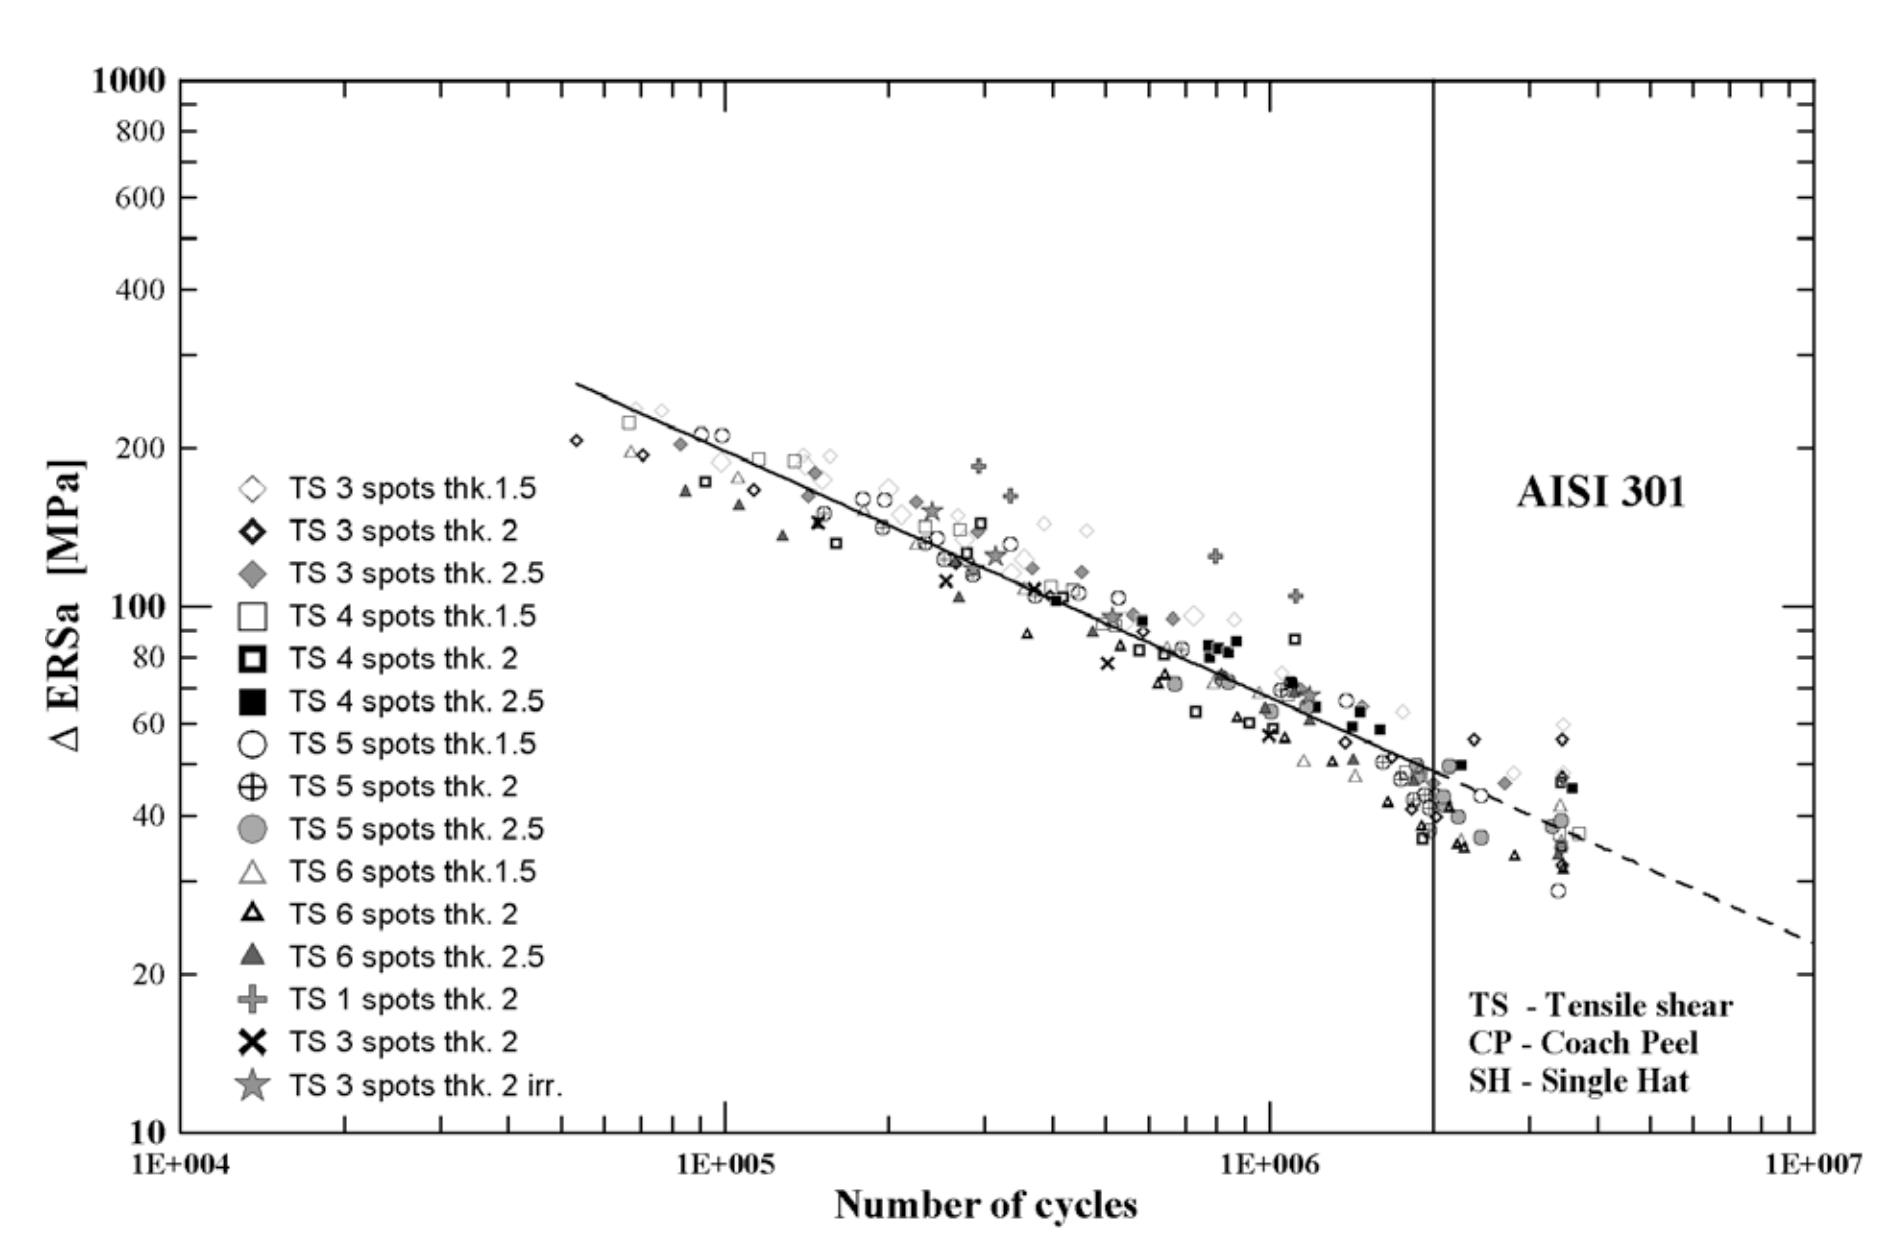
\includegraphics[width=0.5\linewidth]{immagini/screenshot016}
			\label{fig:screenshot016}
		\end{figure}
		Questo accoppia la rotazione intorno al suo asse a quella intorno all'asse del rocchetto, avendo il creatore una forma elicoidale, accoppia sia il moto di accostamento per scavare il dente, sia l'avanzamento assiale: ruotando l'elicoide l'utensile oltre ad avanzare in direzione parallela all'asse avanza anche in direzione ortogonale all'asse. \newline
		
		La condizione limite per non avere interferenza tra rocchetto e dentiera è quella per cui della formula del numero minimo di denti intagliabile il rapporto di trasmissione vale $\tau=0$, tale concetto si ripete similmente sia per creatore che per stozzatrice. 
		
		Tuttavia per la stozzatrice è ancor più semplice individuare il numero minimo di denti, infatti essendo questa di forma circonferenziale (una ruota dentata tagliente), il numero minimo di denti si può individuare a partire dal rapporto di trasmissione tra stozzatrice e rocchetto, questo infatti è il semplice rapporto tra le due circonferenze nella fase di taglio. 

		Nel caso di dentiera e creatore lo si deve invece leggere SEMPRE per $\tau=0$. \newline 
		
		Si è individuato così il limite minimo di denti al fine di scongiurare l'interferenza di taglio, tuttavia  l'interferenza di taglio è interessante perché permette di perdere quella parte di segmento (piccolissima (1) in immagine sottostante) che sarebbe troppo prossima alla circonferenza fondamentale e quindi comporterebbe usura eccessiva.
		\begin{figure}[H]
			\centering
			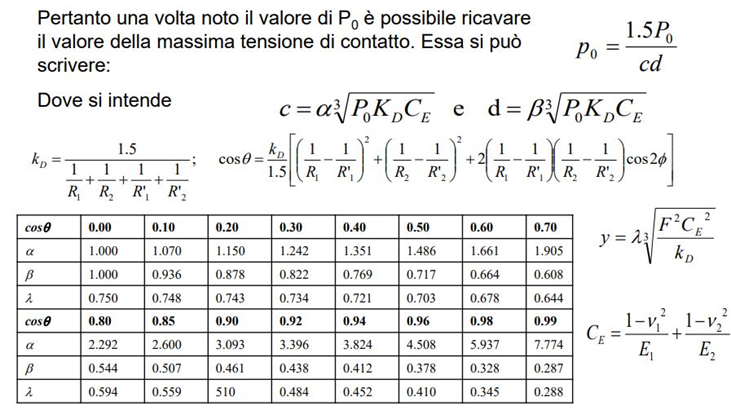
\includegraphics[width=0.5\linewidth]{immagini/screenshot017}
			\label{fig:screenshot017}
		\end{figure}
		Al tempo stesso questa perdita di segmento porta ad avere una riduzione della base del dente.
		
		La normativa DIN fornisce un  numero di riferimento pratico: si può scendere fino a $5\over6$ del numero minimo teorica di denti.
		\[	z_{min}^\text{pratico} = {5\over6}z_{min} = {5\over6}\dfrac{2k'}{\sin^2\theta} \]
		Questa è una regola pratica che porta ad avere  un numero di denti del pignone minore di quello teorico, quindi si avrà una trasmissione più compatta, avendo leggermente scavato la base del dente, così da non avere eventuale contatto in prossimità della circonferenza fondamentale, eludendo il problema dell'usura eccessiva, facendo sempre attenzione al fatto che l'ultimo punto di contatto utile è il punto (C) e quindi sarà la circonferenza passante per quel punto ad assumere il significato di troncatura interna del pignone, quella che effettivamente dà il limite sull'effettivo segmento dei contatti. \newline 
		
		Ovviamente il fattore di ricoprimento può risentire di questa scelta ed è sempre necessario verificare che si maggiore dell'unità. 
		
		In realtà per venire incontro a problemi di imprecisione, montaggio e funzionamento, si preferisce un limite di 1.2 o 1.3 per ruote lente mentre di 1.4 o 1.5 per ruote veloci. 
		
		Durante il funzionamento, se $\varepsilon = 1$, il dente in presa è inflesso dal carico che subisce, nel momento in cui viene rilasciato torna alla posizione iniziale comportando una piccola accelerazione angolare della ruota dentata, poiché il dente in presa è soltanto uno, se sta iniziando in quel momento un nuovo contatto tra denti si avrà giocoforza un urto, problematico ai fini dell'usura e della resistenza del dente; se invece $\varepsilon>1$ c'è più di un dente in presa e ci si mette al riparo da questa tipologia di problemi. \newline 
		
		Il fattore di ricoprimento è strettamente legato al numero di denti delle ruote, infatti il massimo teorico valore di $\varepsilon$ è dato da rapporto tra il massimo segmento dei contatti ed il passo:
		\[\varepsilon = \dfrac{(R+R')\sin\theta}{p\cos\theta} = \dfrac{z+z'}{2\pi}\tan\theta\]
		Se a questo punto si impone $\varepsilon\geq1$ si ottiene che il numero minimo di denti - inteso come somma tra quelli delle due ruote - dev'essere pari a
		\[(z+z')_{min} = 2\pi\cot\theta\]
		
		Si ricordi però che per venire incontro alla condizione di non interferenza si può manipolare l'angolo di pressione prestando sempre attenzione al fatto che un angolo di pressione elevato premette sì di ottenere una ruota dentata più compatta, perché riduce il numero minimo di denti intagliabile, ma sovraccarica maggiormente gli alberi.
		
		In più un angolo di lavoro elevato, porta al problema del dente a punta: alla base il dente è molto robusto e resistente mentre in punta è molto fine ed appuntito, questo porta giocoforza a problemi di urto e ingranamento portando a rigature dei profili. 
		
		Il limite minimo dello spessore del dente in testa è il 20\% del modulo. 
\begin{figure}[H]
	\centering
	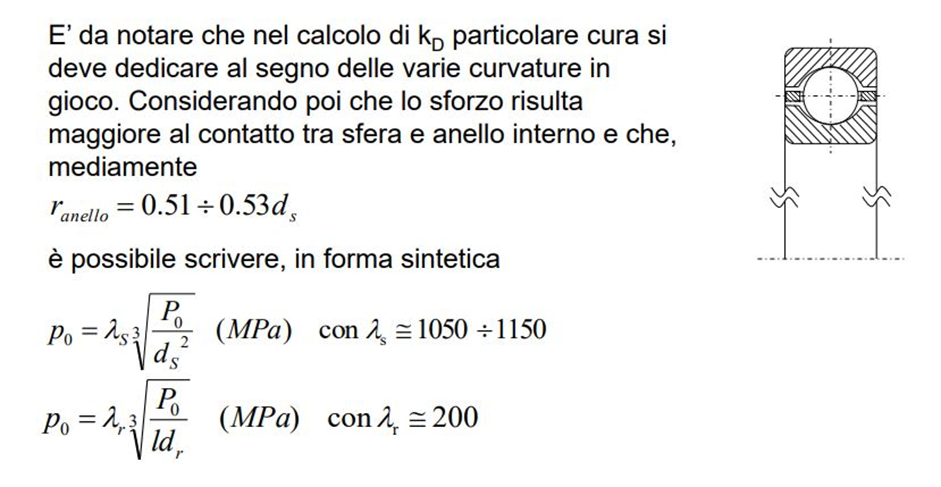
\includegraphics[width=0.5\linewidth]{immagini/screenshot018}
	\label{fig:screenshot018}
\end{figure}		
		Al contrario, un angolo di pressione inferiore ai $20^\circ$ è molto efficiente dal punto di vista della trasmissione dei carichi - carica di meno l'albero - ma porta ad un inviluppo del dente molto ristretto alla base, comportando una minore resistenza di base. 
		
		Seppur l'unificazione consiglia $\theta = 20^\circ$, si trovano valori accettabili anche per $\theta = (15\div30)^\circ$. 
\end{adjustwidth}		 
\subsubsection{Troncatura inferiore}	
\begin{adjustwidth}{2in}{} 	
		L'obiettivo è quello di quantificare il segmento dei contatti perso durante il taglio. 
		
		Come detto infatti nel momento in cui si è deciso di tagliare un numero minimo di denti inferiore a quello minimo di non interferenza - al fine di eliminare quella parte di evolvente in prossimità della fondamentale - si deve mettere in conto una perdita del segmento dei contatti. 
		
		L'obiettivo quindi è quello di individuare la circonferenza passante per l'ultimo punto di evolvente sopravvissuto. 
		\begin{figure}[H]
			\centering
			
\includegraphics[width=0.8\linewidth]{immagini/screenshot019}
			\label{fig:screenshot019}
		\end{figure}
		Si immagini a questo fine un accoppiamento tra una dentiera - la cui primitiva è la retta orizzontale tratto punto che passa per C - ed una circonferenza primitiva di un rocchetto - che in questa immagine non viene riportata ma passerebbe per C -, il profilo della dentiera è individuato dal segmento BA. 
		
		Il dente della dentiera sporge della primitiva di una quantità che è pari all'addendum della dentiera (ovvero al dedendum del dente scavato $5\over4$ in un proporzionamento unificato). 
\begin{figure}[H]
	\centering
	\label{fig:screenshot020}
	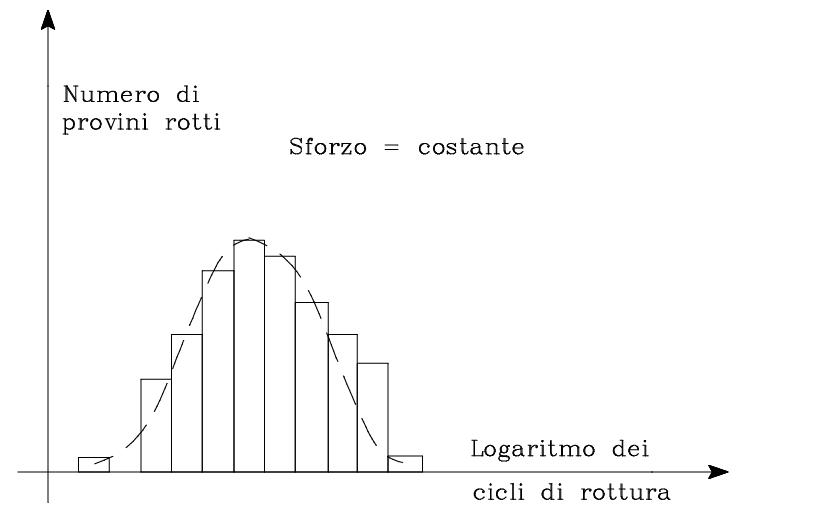
\includegraphics[width=0.5\linewidth]{immagini/screenshot020}
\end{figure}		
		Com'è noto, una parte del dente scava l'evolvente mentre la sua punta scava il raggio di piede della ruota dentata.
		
		Per cui $h = {1\over4}$ del dente della dentiera scava il raggio di raccordo - quello che farà da gioco nel funzionamento - mentre il resto ${5\over4}m -{1\over4}$ sarà la parte utile allo scavo dell'evolvente, in modo che 
		\[u'- h = m \]
		Il punto di contatto tra la testa del dente ed il profilo ad evolvente è l'intersezione fra questa sporgenza del dente della dentiera ed il segmento  dei contatti: i due profili hanno un cinematismo che si incontra nel punto H. 
		
		Il contatto tra il profilo del dente ed il profilo della dentiera invece avviene nel punto P, in quel punto la testa della dentiera tocca per la prima volta il profilo del dente da intagliare.
		
		Questo punto però non appartiene alla retta dei contatti, se questi  fossero due profili coniugati, il contatto dovrebbe avvenire in H, in realtà sta avvenendo in un punto  completamente al di fuori del segmento ei contatti, infatti in P sta avvenendo un contatto per interferenza, l'interferenza di raccordo. \newline 
		
		\textbf{Come si può individuare il cinematismo che avviene durante l'interferenza?}
		
		Il profilo ad evolvente che interseca il profilo della dentiera utensile in P è un profilo che teoricamente rientrerebbe da P arrivando sulla circonferenza fondamentale (tratto continuo) in A, ultimo punto del profilo ad evolvente che si sta scavando. 
		
		Siccome è un punto di interferenza, nel disegno si dovrà prendere in considerazione il suo simmetrico, cioè quel punto individuato sull'evolvente tratteggiata che parte sempre da A ma ora viene costruita in senso orario, su questo tratto la tangente al profilo è individuata dal profilo della dentiera, si ottiene così il punto B, punto di contatto coniugato tra dentiera ed evolvente di circonferenza.  
		\begin{figure}[H]
	\centering
	
\includegraphics[width=0.5\linewidth]{immagini/screenshot019}
	\label{fig:screenshot019.1}
\end{figure}		
		Questo punto è una rulletta del contatto tra profili coniugati che NON sono profilo ad evolvente del dente e fianco della dentiera, ma è il contatto tra il simmetrico del profilo del dente ad evolvente ed il fianco della dentiera, quindi un contatto anomalo tra due profili coniugati. 
		
		Il dente dell'utensile genererà comunque una dentatura ad evolvente perché anche se sta funzionando per interferenza l'inviluppo a cui si dà vita è sempre quello: il rotolamento senza strisciamento della dentiera sul rocchetto. 
		
		Il funzionamento sarà quindi dettato da un accoppiamento tra il fianco della dentiera con un'evolvente simmetrica, non quella reale del dente.\newline 
		
		Si nota immediatamente che B appartiene alla retta dei contatti e quindi il coniugio è verificato. 
		
		Se si individua B' come punto di contatto tra i due profili coniugati (evolvente della ruota e fianco rettilineo della dentiera) relativo al dente successivo appena verificato, allora la distanza BB' sarà per definizione pari al passo, ovvero la dimensione dell'arco tra A e A', dove A' è dove finirebbe l'evolvente del dente già scavato, successivo a quello considerato. \newline
		
		Il tratto di profilo ad evolvente che si sta scavando via è pari all'arco PA, conseguentemente - per proprietà dell'evolvente - si perde una lunghezza del segmento dei contatti pari alla distanza PK.  
		
		K è il punto  individuato dalla normale al profilo P tangente alla circonferenza fondamentale, in pratica quel punto P nell'equazione dell'evolvente era individuato da un angolo $\varphi$, tale angolo moltiplicato per il raggio fondamentale diviene pari all'arco KA, ovvero, per proprietà dell'evolvente, è pari al segmento PK. 
		
		Individuando una traslazione di un certo arco di questo dente tanto da portare il punto P nella posizione T, intersezione della circonferenza di raggio OP con il segmento dei contatti, si individua un dente completamente scavato, in grado di funzionare, e P prende così il ruolo di ultimo punto del segmento dei contatti reale.  
		
		\textbf{E allora il segmento dei contatti perso} sarà il tratto NT. \newline 
		
		Questo tratto NT altro non è che $\rho\varphi$, conoscendo l'angolo $\varphi$ si riesce ad individuare quanto segmento di contatti è potenzialmente perso, nella pratica, quanto effettivamente è perso non dipende da quanto è stata scavata la ruota, ma da quanto si accoppia la ruota coniugata: è la troncatura esterna dell'altra ruota che indica l'ultimo punto  effettivo di contatto. 
		
		Per cui, ricapitolando, in formule: 
		\[PK = \rho\varphi = \overset{\huge\frown}{KA} = NT\] 
\end{adjustwidth}		
		\subsubsection{Individuazione di $\varphi$}
\begin{adjustwidth}{2in}{} 
		Per trovare $\varphi$  la dimostrazione è ancora una volta di tipo geometrico. 
		
		Si deve proiettare su una retta ON - radiale - e su una retta ortogonale a questa CN  - segmento dei contatti - le quantità OK, KB, PB. \newline 
		
		OK proiettato su CN è pari a $\rho\sin\gamma$ dove $\gamma = \varphi + \psi$ e $\varphi$ è l'incognita, la posizione angolare rispetto a K di P e $\psi$ è l'angolo che manca per arrivare a ON. 
		
		KP è pari a $\rho\varphi$, proiettato su CN avrà un'estensione pari a $\rho\varphi\cos\gamma$: PK e OK sono perfettamente ortogonali tra loro.  
		
		PB è ortogonale a CN e quindi non dà contributo. 
		
		BO ha invece un'estensione in direzione CN pari a $\rho\psi$.
		\[\rho\sin\gamma - \rho\psi\cos\gamma - \rho\psi = 0\]
		
		OK proiettato sulla retta ON è pari a $\rho\cos\gamma$. 
		
		KP proiettato sulla retta ON è pari a $\rho\psi\sin\gamma$. 
		
		PB si quantifica dalla relazione seguente. 
		
		Se BH è pari a  $\rho(\lambda-\psi)$ dove $\lambda$ è un parametro arbitrario tale che moltiplicato per $\rho$ dia la distanza NH, per cui si individua un triangolo rettangolo HBP di ampiezza pari all'angolo di pressione, e allora PB sarà nient'altro che $\rho(\lambda-\psi)\tan\theta$. 
		
		BO proiettato in direzione ON non è altro che ON, e quindi è pari a $\rho$.
		\[\rho\cos\gamma + \rho\psi\sin\gamma +  \rho(\lambda-\psi)\tan\theta - \rho\]
		
		Per cui, infine si ha		
		\[\begin{cases}
			\sin\gamma - \psi\cos\gamma = \psi \\
			\cos\gamma + \psi\sin\gamma +  (\lambda-\psi)\tan\theta = 1
		\end{cases}\]
		Questa due relazioni, posto $\gamma = \varphi + \psi$ forniscono due formule
		\[\varphi = \dfrac{\gamma - \sin\gamma}{1-\cos\gamma} \qquad \lambda = (1-\cos\gamma-\varphi\sin\gamma)\cot\gamma + (\gamma-\varphi)\]
		Ad angolo di pressione fissato il tutto si riduce a 
		\[\varphi = \varphi(\lambda)\]
		Ricordando che $\varphi$ è l'incognita di partenza, quella che moltiplicata per $\rho$ fornisce il segmento di contatti perso. 
		
		Per come è stato definito $\lambda$, questo è pari a 
		\[\lambda = \dfrac{HN}{\rho} = \dfrac{1}{\rho}\left[\dfrac{u'-h}{\sin\theta} - \rho\tan\theta\right] = \dfrac{4}{z\sin(2\theta)} \dfrac{u'-h}{m} - \tan\theta\] 
		Ovvero funzione della sporgenza utile dell'utensile $u'- h$. 
		
		Dove si sono usate le già viste relazioni
		\[\rho = R\cos\theta \qquad p = \dfrac{2\pi R}{z} = m\pi \Rightarrow R = \dfrac{zm}{2}\] 		
		Riportando in un grafico questa relazione geometrica:
		\begin{figure}[H]
			\centering
			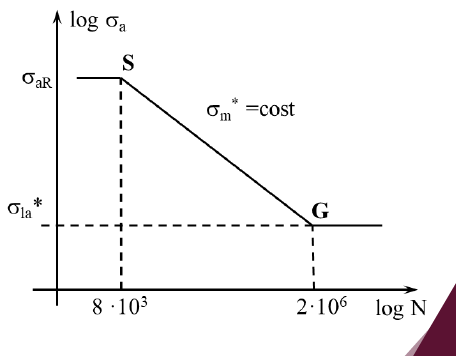
\includegraphics[width=0.5\linewidth]{immagini/screenshot021}
			\label{fig:screenshot021}
		\end{figure}
		Si ottiene l'incognita $\varphi$ al variare dell'angolo di pressione $\theta$ in funzione del valore di $\lambda$. 
		
		Ottenendo finalmente di quanto si sposta sul segmento dei contatti, l'ultimo punto utile di contatto.
\end{adjustwidth}
\newpage	
\section{Strisciamento specifico ed usura}
\begin{adjustwidth}{2in}{}
	Per quale motivo si riduce principalmente il segmento dei contatti? 
	
	Perché si vuole evitare l'usura. \newline 
	
	Prima ancora di parlare di usura, bisogna prevedere una grandezza cinematica importante: lo strisciamento specifico tra i profili. 
	
	Si sono già descritti i vettori velocità, infatti nel moto istantaneo relativo di rotolamento senza strisciamento di una primitiva sull'altra, il centro di istantanea rotazione C, è il centro intorno al quale avviene una rotazione relativa $\bar{\omega}$ che è l'atto di rotolamento senza strisciamento di una  circonferenza sull'altra, per cui il punto di contatto M è  dotato di una velocità relativa centrata in C, quindi ogni punto di contatto M ha un vettore di moto relativo di un profilo sull'altro, proprio per definizione. 
	
	La velocità relativa $\bar\omega^*$ è la differenza tra le $\omega_i$ mentre il vettore velocità relativa è pari a 
	\[\vec{v}_{12} = (C-M)\times\bar\omega^*\]
	Vettore sempre ortogonale alla retta dei contatti. 
	
	Siccome i profili sono tangenti e hanno normale nel punto dei contatti pari al segmento dei contatti, vuol dire che questa velocità relativa è sempre ortogonale al profilo, e quindi è uno  strisciamento. 
	
	Questa velocità relativa sarà nulla in C, centro di  istantanea rotazione, unico punto dove non c'è strisciamento specifico, ma più ci si distanzia da C lungo il segmento dei contatti e maggiore sarà lo strisciamento specifico. 
\begin{figure}[H]
	\centering
	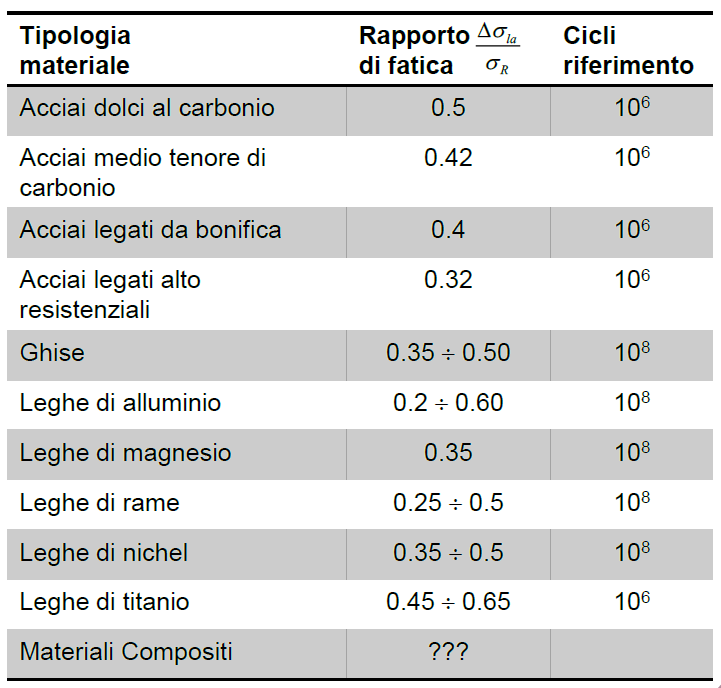
\includegraphics[width=0.5\linewidth]{immagini/screenshot022}
	\label{fig:screenshot022}
\end{figure}
	Siccome sono profili coniugati ad evolvente, avranno la stessa componente normale al profilo, $\vec{v}_n$, ma hanno diverse velocità tangenziali al profilo, la differenza tra queste due velocità è la $\vec{v}_{12}$. \newline 
	
	È necessario quantificare gli aspetti di questa velocità tangenziale ai profili perché porta, durante all'ingranamento a strisciamenti specifici. 
	
	Infatti se si vedesse nello spazio fisso il punto di contatto, questo si muoverebbe lungo il segmento dei contatti, ma se istante per instante si guardasse il punto del profilo attivo che sta svolgendo il ruolo di contatto e si andasse a misurare tra due istanti successivi di quanto si sia mosso sul profilo della ruota e su quello del pignone, quella distanza - che in un'ascissa curvilinea lungo l'evolvente prende il nome di $ds$ e $ds'$ -  è differente.
	
	Questo perché l'entità dello spostamento lungo il profilo del dente è dettata dalla sola componente tangenziale al profilo, che è diversa su ruota e su pignone. 
	
	In termini adimensionali questa differenza di spostamento si chiama \textbf{strisciamento specifico}. \newline
	
	Questo strisciamento è dato, rispettivamente su ruota motrice e ruota condotta da: 
	\[\begin{dcases}
		k_s  = \dfrac{ds-ds'}{ds} \\
		k_s' = \dfrac{ds'- ds}{ds}
	\end{dcases}\]
	La relazione geometrica che fornisce gli strisciamenti specifici si individua a partire dalla scomposizione della velocità angolare relativa. 
	
	Il moto relativo avviene istante per istante intorno a C con velocità relativa data dalla composizione vettoriale delle $\omega_i$ ed i profili dei denti hanno un moto di rotazione $\bar{\omega}$ intorno ai loro centri di curvatura $\Omega, \Omega'$, questi individuati esattamente nei punti di tangenza tra il segmento dei contatti con le circonferenze fondamentali ($T, T'$). 
	
	Per traslazione, sfruttando le proprietà dei moti, la velocità $\bar{\omega}$ intorno al centro di curvatura sarà data dalla velocità relativa per il rapporto tra le distanze dei centri di curvatura
	\[\bar{\omega} = (\omega_1 + \omega_2)\dfrac{C\Omega'}{\Omega\Omega'} \qquad \bar{\omega}' = (\omega_1 + \omega_2)\dfrac{C\Omega}{\Omega\Omega'}\]
	Lo spostamento in direzione tangenziale al profilo $ds$ sarà un atto di moto intorno al centro di curvatura, ovvero 
	\[ds = \bar{\omega}\cdot\Omega M\cdot dt \qquad ds' = \bar{\omega}'\cdot\Omega' M\cdot dt \]
	Gli strisciamenti specifici assumono così la seguente formulazione 
	\[k_s = \dfrac{CM}{\Omega M} \cdot \dfrac{\Omega\Omega'}{C\Omega'} \qquad k_s' = \dfrac{CM}{\Omega' M} \cdot \dfrac{\Omega\Omega'}{C\Omega}\]
	Si è trovata così una formulazione che lega gli strisciamenti specifici alle grandezze geometriche in atto, per cui, ci si riconduce facilmente a 
	\begin{eqnarray}
		k_s = (1+\tau)\dfrac{\delta}{R\sin\theta +\delta} \\
		k'_s = -\left(1+\dfrac{1}{\tau}\right)\dfrac{\delta}{R'\sin\theta -\delta}
	\end{eqnarray}
	Dove si sono poste 
	\[CM = \delta\]
	Ascissa curvilinea definita come distanza del punto di contatto dal centro di istantanea rotazione.
	\[\Omega M = CM + C\Omega = \delta + R\sin\theta\]
	Gli strisciamenti specifici sono così funzioni dipendenti da:
	\begin{itemize}
		\item Specifico punto in cui sta avvenendo l'ingranamento $\delta$ 
		\item Rapporto di trasmissione $\tau$
		\item Angolo di pressione $\theta$
	\end{itemize} 
	Tutte grandezze geometriche e caratteristiche della trasmissione. 
\newpage	
	Ciò che si ottene da queste funzioni strisciamento non è un singolo valore, ma una funzione al variare di $\delta$ che traccia un andamento di questo tipo
	\begin{figure}[H]
		\centering
		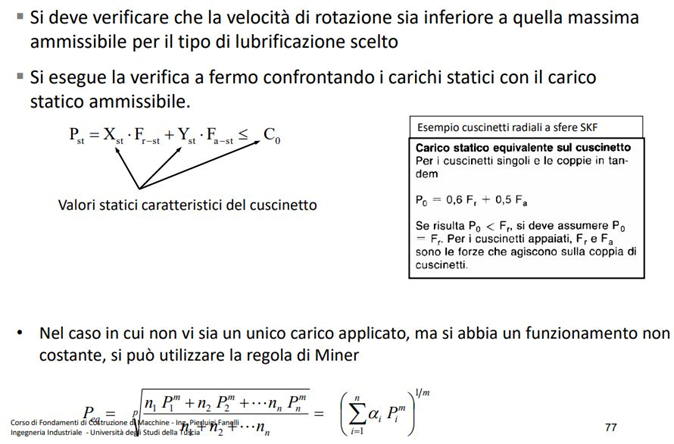
\includegraphics[width=0.5\linewidth]{immagini/screenshot023}
		\label{fig:screenshot023}
	\end{figure}
	Con $\delta$ che va da [-segmento di accesso a + segmento di recesso]. 
	
	\textbf{OSSERVAZIONI} \\
	In C gli strisciamenti sono nulli. 
	
	Per la ruota motrice si individua un valore negativo da una parte ed un valore negativo che tende ad infinito dell'altra. 
	
	Per la condotta si individua un valore - infinito da una parte  ed un valore positivo finito dall'altra.
	
	Gli strisciamenti specifici tendono ad infinito in T e T', potenziale contatto sulla base dell'evolvente, ecco perché si deve evitare il contatto in quel punto, perché semmai dovesse avvenire, si va incontro a strisciamenti infiniti. 
	
	Nella realtà non saranno mai T e T' da tenere d'occhio, ma K e K', estremità del segmento effettivo dei contatti, andando ad osservare le troncature esterne di ruota e pignone, significherà quindi un diagramma degli strisciamenti specifici ristretto ad una zona dove non tendono più ad infinito. 
	
	\textbf{ATTENZIONE} Si vede subito che lo strisciamento è sbilanciato verso la ruota più piccola, il pignone. 
	
	Come si può agire? 
	
	\begin{itemize}
		\item Scavando la base: si sposta la troncatura interna più in alto rispetto alla base dell'evolvente. 
		
		Il segmento dei contatti diminuisce insieme all'ampiezza del grafico. 
	\end{itemize}
	
	Gli strisciamenti devono essere tenuti sotto controllo dal punto di vista dei moduli dei valori massimi, che dev'essere sempre inferiore al valore di progetto di 1.4, e devono inoltre essere equilibrati, l'equilibratura degli strisciamenti si effettua agendo esclusivamente in fase di taglio attraverso la correzione della dentatura, spostando le circonferenze primitive di taglio in modo opportuno.  	
	
	(Quando cambio una ruota in un ingranaggio cambio sempre l'intero ingranaggio: ruota e pignone.) 
	
	
	
	
	
	
	
		
	
		
		
		
		
		
		 
		
		   
		
		
		
		

	   
	   
	   
	   
	   
	   
		
		
	    
 
	    
	    
	    
	    
	    
	   
	     
	     
	     
	     
	
	
	
	
	
	
	
	
	
	
	
	
	
	
	
	
	\newpage
	\textbf{{\LARGE NOTE}}
%	\vfill
%	\begin{tcolorbox}[height=4.5cm]
%		This box has a height of 4.5cm.
%	\end{tcolorbox}
	
	%DA DECOMMENTARE PER AVERE LA VERSIONE STAMPABILE A DUE PAGINE 	
	%	\newpage
	%		\null
	%		\vfill
	%\begin{tcolorbox}[height=4.5cm]
	%	This box has a height of 4.5cm.
	%\end{tcolorbox}
	%		
\end{adjustwidth}
\end{document}